\section {Análise}

Esta seção é dedicada às características que determinam as três montagens.

\subsection{Criação do Projeto}

Com base no tutorial fornecido em [\ref{bib:tutorial}], foi possível
realizar um projeto capaz de piscar o \textit{LED} vermelho, conectado ao pino
\textbf{PTB18}, a uma frequência de 1Hz. A fim de extendê-lo para também piscar
o verde, adicionamos um outro pino \textit {BitIO} de entrada ou saída, a partir
da aba \textit{Components Library}, e o configuramos de acordo com a informações
contidas em [\ref{bib:manual}] sobre o \textit{LED} verde. No campo \textit{Pin
for I/O}, introduzimos o pino \textbf{PTB19} e, posteriormente, geramos a função
\textit{NegVal} da mesma maneira que geramos para o vermelho. Para fazê-lo
piscar a uma frequência de 2Hz, utilizamos o mesmo \textit{timer} \textit{T1},
no entanto alteramos o período de geração de interrupções para 250\textit{ms}.
Na função tratadora da interrupção, introduzimos uma variável inteira
persistente (\textit{static}), isto é, seu valor será conservado ao fim da
função e poderá ser acessado em outras chamadas, cujo valor será 0 ou 1 e, a
cada interrupção tem seu conteúdo negado. Quando tal variável vale 0, os dois
\textit{LEDs} estão acesos e quanto vale 1, somente o verde se acende. Dessa
forma, o \textit{LED} vermelho permanecerá acesso ou apagado por 2 interruções,
isto é, por 500\textit{ms}, tendo assim um período de 1\textit{s}. O verde
muda de estado a cada 250ms, obtendo, portanto, um período de 500ms.

\vspace{12pt}

As funcionalidades acima podem ser resumidas em diagramas de blocos funcionais.
Para a configuração contendo somente o \textit{LED} vermelho, obtem-se o
seguinte diagrama, em que blocos em azul são implementados como circuito
elétricos (\textit{hardware}) e, em vermelho, como \textit{software}: 

\FloatBarrier

\begin{figure}[h]
    \centering
    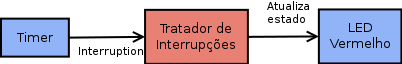
\includegraphics[scale=0.7]{image/montagem1}
    
    \caption{Diagrama para a primeira montagem.}
    \label{fig:m1}
\end{figure} 

\FloatBarrier

O \textit{timer} é um circuito que possui um registrador que realiza contagens
a cada ciclo de \textit{clock}. Quando a contagem chega a um limite, que é
calculado em função do intervalo de tempo desejado, uma interrupção é lançada
para o processador. O tratador desta interrupção é uma função, escrita em
linguagem de alto ou baixo nível, cujo propósito é reagir ao ``estímulo''. No
nosso caso, tal rotina chamará outras funções capazes de alterar o estado lógico
dos \textit{LEDs}. O estado lógico precisa ser convertido em características
físicas, como corrente e tensão, já que os \textit{LEDs}, sendo diodos, são
componentes de um circuito elétrico. Observa-se que o único bloco constituído de
\textit{software} realiza um papel centralizador e controlador dos módulos
\textit{hardware}, o que permite ao programador uma grande liberdade e escolhas
de programação.

\vspace{12pt}

Para a montagem com o \textit{LED} verde:

\FloatBarrier

\begin{figure}[h]
    \centering
    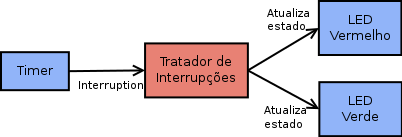
\includegraphics[scale=0.7]{image/montagem2}
    
    \caption{Diagrama para a segunda montagem.}
    \label{fig:m2}
\end{figure} 

\FloatBarrier

O diagrama é muito parecido com aquele presente na figura \ref{fig:m1}. Isto
quer dizer que é possível utilizarmos praticamente os mesmos componentes
utilizados na montagem anterior e configurar somente os parâmetros que
necessitam ser alterados, como, por exemplo, o período de geração de
interrupções.

\subsection{Conexão de LED externo}

A primeira etapa para a conexão de um \textit{LED} externo é a escolha da porta
que funcionará como saída e que fornecerá a corrente necessária para que ele se
acenda. Tal escolha foi baseada na posição das conexões dos pinos nos
\textit{headers} da placa, de acordo com [\ref{bib:userguide}], e na
disponibilidade  do respectivo pino de funcionar como \textit{output}. Sendo
assim, por estar na primeira linha e na primeira coluna do \textit{header} da
esquerda, facilitando assim a sua identificação na placa auxiliar da FEEC,
escolhemos o pino \textbf{PTA1}. Adicionamos, posteriormente, um novo componente
\textit{BitIO} ao projeto e o configuramos para refletir a escolha acima.
Modificamos o campo \textit{Init. value} para 1, a fim de que o \textit{LED}
externo já se acenda assim que o programa for lançado.

\vspace{12pt}

Antes de realizarmos a montagem do circuito, é necessário considerar as
correntes e tensões máximas suportadas pelos componentes, cujos valores
são descritos nos \textit{datasheets} do microcontrolador
[\ref{bib:datakl25}] e do \textit{LED} externo [\ref{bib:led}]. Para o primeiro,
as linhas 1 e 3 a tabela 7 especificam, respectivamente, que a tensão mínima
fornecida no pino em estado lógico alto é \(V_{DD} - 0,5\), isto é, 3.3V, e que
a corrente máxima total de todas as portas é 100mA. Considerando, que
utilizaremos somente uma porta, o valor máximo de corrente suportada pelo
microcontrolador é, portanto, 100mA. Para o \textit{LED}, [\ref{bib:led}] nos
diz que a corrente DC direta máxima vale 50mA e que a maior tensão reversa
suportada é 6V. Sendo assim, adotaremos um limiar máximo para a corrente de
\textbf{50mA}.

\vspace{12pt}

Considerando o valor mínimo de tensão no pino de saída do microcontrolador, isto
é, \(V_{pin}=3.3V\), a figura 5 do \textit{datasheet} do \textit{LED}, que
especifica uma relação diretamente entre corrente \(i\) e tensão direta
\(V_{LED}\), e a relação \(i=\frac{V_{pin} - V_{LED}}{R}\), podemos escolher um
resistor de \(100\Omega\). Obtemos, portanto, uma corrente de aproximadamente
13mA. 

\vspace{12pt}

É importante notar que utilizamos o pino terra da própria placa, isto é, o
pino \textbf{GND}, presente no 14º pino do \textit{header} inferior esquerdo da
figura da página 12 de [\ref{bib:datakl25}].

\vspace{12pt}

O diagrama desta montagem é muito simples: logo que o programa é iniciado, o
\textit{LED} externo é aceso. O bloco \textit{LED Externo} engloba todo o
circuito (resistência, diodo, fios) que foram necessários para a sua
implementação. Observa-se igualmente que este bloco poderia ser facilmente
substituído por um dos blocos \textit{LED vermelho} ou \textit{LED verde} das
figuras \ref{fig:m1} e \ref{fig:m2}. Esta característica demonstra que programas
feitos para este microcontrolador não dependem estritamente de componentes
específicos, isto é, são capazes de garantir soluções genéricas que funcionam
para diversos tipos de \textit{hardware} distintos, em termos de tensão,
corrente, potência \textit{etc}.

\FloatBarrier

\begin{figure}[h]
    \centering
    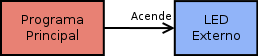
\includegraphics[scale=0.7]{image/montagem3}
    
    \caption{Diagrama para a terceira montagem.}
    \label{fig:m3}
\end{figure} 

\FloatBarrier

\subsection{Chave de controle}

A última montagem envolve a utilização de um pino de entrada e de um
\textit{push button}, cuja função é controlar a atividade dos \textit{LEDs}, de
forma a permitir que eles pisquem quando o botão estiver apertado e apagá-los,
caso contrário. Para isso, utilizamos um circuito representado na figura
\ref{fig:circ} a seguir, em que \textbf{P3V3} é um pino que fornece uma tensão
de 3.3V, \textbf{GND} é a referência do terro na placa e \textbf{PTD4} é o pino
escolhido como \textit{input}.

\begin{figure}[h]
    \centering
    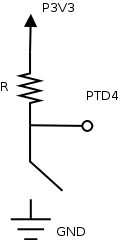
\includegraphics[scale=0.7]{image/circuito}
    
    \caption{Circuito utilizado na montagem.}
    \label{fig:circ}
\end{figure} 

O resistor \textbf{R} é chamado de \textit{pull up resistor}, visto que ele
induz um estado padrão alto na saída do circuito, isto é, \textbf{PTD4}. O
circuito pode apresentar dois comportamentos distintos, dependendo do
estado da chave. Quando está aberta, praticamente há não passagem de
corrente entre \textbf{P3V3} e \textbf{PTD4}, já que a impedância de entrada do
pino de entrada é elevada. Por esta razão, o nível lógico deste
pino é alto nesta configuração. Em oposição, quando a chave é fechada
(\textit{push-button} pressionado), \textbf{PTD4} conecta-se ao terra e,
portanto, adquire um nível lógico baixo.

\vspace{12pt}

O valor de \textbf{R} deve garantir as especificações de corrente máxima do
fabricante. Sendo assim, utilizamos uma resistência de \(1k\Omega\), que
garantirá uma corrente de aproximadamente 3.3mA passando pelo circuito quando a
chave estiver fechada.

\vspace{12pt}

Por fim, adicionamos um novo componente \textit{BitIO} ao projeto, o
configuramos para referenciar \textbf{PTD4} e funcionar como \textit{input}.
Geramos, em seguida, a função \textit{GetVal}, cujo valor de retorno é o estado
lógico do respectivo pino. A cada interrupção do \textit{timer}, chamaremos tal
função para determinar se o botão foi pressionado ou não. Se o retorno for nulo,
isto é, botão apertado, piscamos os \textit{LEDs}, conforme seções anteriores.
Senão, os apagaremos colocando níveis lógicos altos em \textbf{PTB18} e
\textbf{PTB19}.

\vspace{12pt}

O diagrama da última montagem é representado na figura \ref{fig:m4}. O bloco
\textit{push button} engloba todo o circuito representado pelo figura
\ref{fig:circ}.

\FloatBarrier

\begin{figure}[h]
    \centering
    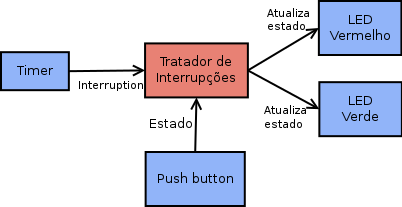
\includegraphics[scale=0.7]{image/montagem4}
    
    \caption{Diagrama para a quarta montagem.}
    \label{fig:m4}
\end{figure} 

\FloatBarrier

Nota-se que a única diferença entre este diagrama e aquele da figura
\ref{fig:m2} é a presença do \textit{push button}. Sendo assim, observa-se uma
grande portabilidade de código e componentes entre diversas aplicações. 
